\section{Funktionen}
Eine Funktion $f: D \rightarrow W$ ist eine Vorschrift, nach der jedem Element aus
$D$ ein Element aus $W$ zugeordnet wird. $D$ ist der \underline{Definitionsbereich}
(Bereich der gültigen Eingaben) und $W$ der \underline{Wertebereich}
(Bereich der gültigen Ausgaben).

Ist $f: M \rightarrow N$ und $g: N \rightarrow P$, so ist die Funktion $g \circ f: M \rightarrow P$,
$(g \circ f)(x) = g(f(x))$, eine \underline{Komposition} von $f$ und $g$.

\subsection{Regeln}
\begin{itemize}
	\item $f(A \cap B) \subseteq f(A) \cap f(B)$
	\item $f(A \cup B) = f(A) \cup f(B)$
\end{itemize}

\subsection{Identität (identische Abbildung, $\id_X$)}
Sei $M$ eine Menge, dann ist die \textit{identische Abbildung von $M$} definiert durch:
$\id_M: M \rightarrow M$ mit $\id_M(x) = x$.

Sei $f: M \rightarrow N$ eine beliebige Funktion, dann gilt:
\begin{itemize}
	\item $\id_N \circ f = f$
	\item $f \circ \id_M = f$
\end{itemize}

\subsection{Injektiv, surjektiv, bijektiv}
\subsubsection{Injektiv}
Sei $f: M \rightarrow N$, $f$ ist injektiv, wenn folgendes gilt:
\begin{itemize}
	\item $\forall x_1, x_2 \in M: x_1 \neq x_2 \Rightarrow f(x_1) \neq f(x_2)$
	\item $\forall x_1, x_2 \in M: f(x_1) = f(x_2) \Rightarrow x_1 = x_2$
	\item $\forall y \in N: \exists !x \in M: f(x) = y \lor \lnot(\exists x \in M: f(x) = y)$: wenn zu jedem $y \in N$ höchstens (genau eins oder keins) ein $x \in M$ existiert mit $f(x) = y$
\end{itemize}

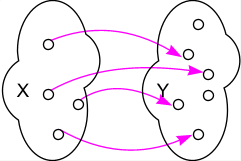
\includegraphics[scale=0.5]{injektiv.png}

\paragraph{Injektivität zeigen}
Injektiv wird meist direkt über die zweite Eigenschaft gemacht oder per Wiederspruchsbeweis (indirekter Beweis) mittels der ersten Eigenschaft bewiesen.
\todo{Beispiel?}

\paragraph{Eigenschaften}
\begin{itemize}
	\item Die Gleichung $f(x) = y$, $f$ ist injektiv und $y$ gegeben, verfügt über eine oder keine Lösung für $x$
	\item Eine \textit{stetige reelwertige} Funktion auf einem \textit{reelen Intervall} ist genau dann \underline{injektiv}, wenn sie in ihrem gesamten Definitionsbereich \textit{streng monoton} steigend oder fallend ist.
	\item Sind die beiden Funktionen $g, f$ injektiv, so ist die \underline{Komposition} $g \circ f$ ebenfalls injektiv
	\item Ist $g \circ f$ injektiv, so ist $f$ injektiv
	\item $f: M \rightarrow N$ ist injektiv, wenn es die \underline{links inverse} Funktion $g: N \rightarrow M$ gibt, so dass $g \circ f = \id_M$
\end{itemize}

\subsubsection{Surjektiv}
Sei $f: M \rightarrow N$, $f$ ist surjektiv, wenn folgendes gilt:
\begin{align*}
\forall y \in N: \exists x \in M: f(x) = y
\end{align*}
Wenn also für jedes Element aus $N$ mindestens ein (können auch mehr sein) Element in $M$ gibt, dass auf das Element aus $N$ zeigt.

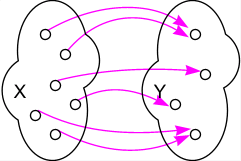
\includegraphics[scale=0.5]{surjektiv.png}

\paragraph{Eigenschaften}
\begin{itemize}
	\item Die Gleichung $f(x) = y$, $f$ ist surjektiv und $y$ gegeben, verfügt über eine oder mehrere Lösungen für $x$.
	\item Sind die Funktionen $f: A \rightarrow B$ und $g: B \rightarrow C$ surjektiv, so ist die \underline{Komposition} $g \circ f: A \rightarrow C$ auch surjektiv
	\item Ist $g \circ f$ surjektiv, so folgt, dass $g$ surjektiv ist
	\item $f: A \rightarrow B$ ist genau dann surjektiv, wenn $f$ ein \underline{rechtes Inverse} hat, also $g: B \rightarrow A$ mit $f \circ g = \id_B$
\end{itemize}

\subsubsection{Bijektiv}
Eine Funktion ist bijektiv, wenn sie injektiv und surjektiv ist.

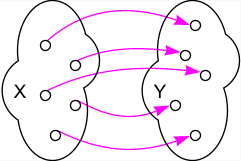
\includegraphics[scale=0.5]{bijektiv.png}

\paragraph{Eigenschaften}
\begin{itemize}
	\item Es gelten die Eigenschaften von Injektivität und Surjektivität
	\item Die Gleichung $f(x) = y$, $f$ ist bijektiv und $y$ gegeben, verfügt über genau eine Lösung für $x$
	\item Sind die Funktionen $f: A \rightarrow B$ und $g: B \rightarrow C$ bijektiv, dann ist auch die \underline{Komposition} $g \circ f: A \rightarrow C$ bijektiv.
	\item Ist $g \circ f$ bijektiv, dann ist $f$ injektiv und $g$ surjektiv
\end{itemize}
